\documentclass[tikz,border=8pt]{standalone}

\usepackage[T1]{fontenc}
\usepackage[utf8]{inputenc}
\usepackage{lmodern}
\usepackage{amsmath}
\usepackage{tikz}
\usetikzlibrary{arrows.meta,positioning,fit,calc,backgrounds}

\begin{document}
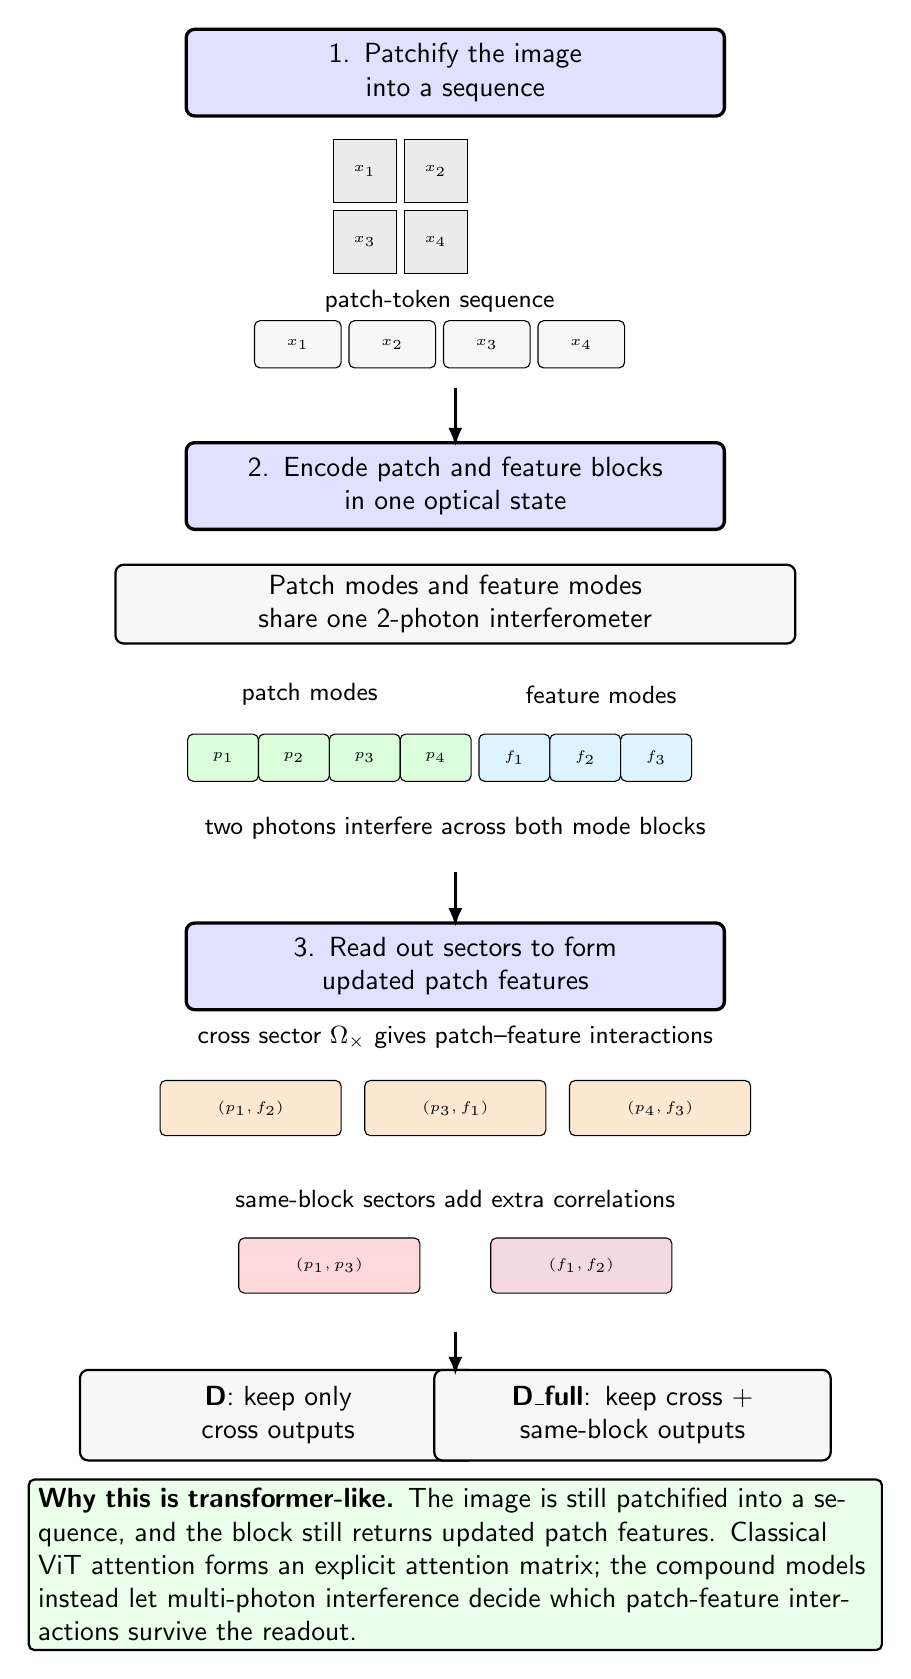
\begin{tikzpicture}[
  font=\sffamily,
  x=1cm, y=1cm,
  patch/.style={draw, minimum width=0.8cm, minimum height=0.8cm, fill=gray!15},
  token/.style={draw, rounded corners=2pt, minimum width=1.1cm, minimum height=0.6cm, align=center, fill=gray!6, thin},
  title/.style={draw, rounded corners=3pt, text width=6.6cm, minimum height=1.1cm, align=center, fill=blue!12, very thick},
  block/.style={draw, rounded corners=3pt, text width=8.4cm, minimum height=1.0cm, align=center, fill=gray!6, thick},
  patchmode/.style={draw, rounded corners=2pt, minimum width=0.9cm, minimum height=0.6cm, align=center, fill=green!14, thin},
  featmode/.style={draw, rounded corners=2pt, minimum width=0.9cm, minimum height=0.6cm, align=center, fill=cyan!14, thin},
  cross/.style={draw, rounded corners=2pt, minimum width=2.3cm, minimum height=0.7cm, align=center, fill=orange!18, thin},
  samep/.style={draw, rounded corners=2pt, minimum width=2.3cm, minimum height=0.7cm, align=center, fill=red!15, thin},
  samef/.style={draw, rounded corners=2pt, minimum width=2.3cm, minimum height=0.7cm, align=center, fill=purple!15, thin},
  decision/.style={draw, rounded corners=3pt, text width=4.8cm, minimum height=1.15cm, align=center, fill=gray!6, thick},
  note/.style={draw, rounded corners=2pt, text width=10.6cm, minimum height=1.0cm, align=left, fill=green!8, thick},
  arrow/.style={-{Latex[length=2.4mm]}, very thick}
]

% step 1
\node[title] (s1) at (5.7, 0.0) {1. Patchify the image\\into a sequence};
\node[patch] (p1) at (4.55, -1.25) {};
\node[patch] (p2) at (5.45, -1.25) {};
\node[patch] (p3) at (4.55, -2.15) {};
\node[patch] (p4) at (5.45, -2.15) {};
\node at (4.55, -1.25) {\tiny $x_1$};
\node at (5.45, -1.25) {\tiny $x_2$};
\node at (4.55, -2.15) {\tiny $x_3$};
\node at (5.45, -2.15) {\tiny $x_4$};
\node[token] (tok1) at (3.7, -3.45) {\tiny $x_1$};
\node[token] (tok2) at (4.9, -3.45) {\tiny $x_2$};
\node[token] (tok3) at (6.1, -3.45) {\tiny $x_3$};
\node[token] (tok4) at (7.3, -3.45) {\tiny $x_4$};
\node at (5.5, -2.9) {\small patch-token sequence};

% step 2
\node[title] (s2) at (5.7, -5.25) {2. Encode patch and feature blocks\\in one optical state};
\node[block] (state) at (5.7, -6.75) {Patch modes and feature modes\\share one 2-photon interferometer};
\node at (3.85, -7.9) {\small patch modes};
\node at (7.55, -7.9) {\small feature modes};
\node[patchmode] (pm1) at (2.75, -8.7) {\tiny $p_1$};
\node[patchmode] (pm2) at (3.65, -8.7) {\tiny $p_2$};
\node[patchmode] (pm3) at (4.55, -8.7) {\tiny $p_3$};
\node[patchmode] (pm4) at (5.45, -8.7) {\tiny $p_4$};
\node[featmode]  (fm1) at (6.45, -8.7) {\tiny $f_1$};
\node[featmode]  (fm2) at (7.35, -8.7) {\tiny $f_2$};
\node[featmode]  (fm3) at (8.25, -8.7) {\tiny $f_3$};
\node at (5.7, -9.6) {\small two photons interfere across both mode blocks};

% step 3
\node[title] (s3) at (5.7, -11.35) {3. Read out sectors to form\\updated patch features};
\node at (5.7, -12.25) {\small cross sector $\Omega_{\times}$ gives patch--feature interactions};
\node[cross] (c1) at (3.1, -13.15) {\tiny $(p_1,f_2)$};
\node[cross] (c2) at (5.7, -13.15) {\tiny $(p_3,f_1)$};
\node[cross] (c3) at (8.3, -13.15) {\tiny $(p_4,f_3)$};
\node at (5.7, -14.3) {\small same-block sectors add extra correlations};
\node[samep] (pp1) at (4.1, -15.15) {\tiny $(p_1,p_3)$};
\node[samef] (ff1) at (7.3, -15.15) {\tiny $(f_1,f_2)$};
\node[decision] (d) at (3.45, -17.05) {\textbf{D}: keep only\\cross outputs};
\node[decision] (df) at (7.95, -17.05) {\textbf{D\_full}: keep cross +\\same-block outputs};
\node[note] (n) at (5.7, -18.95) {\textbf{Why this is transformer-like.} The image is still patchified into a sequence, and the block still returns updated patch features. Classical ViT attention forms an explicit attention matrix; the compound models instead let multi-photon interference decide which patch-feature interactions survive the readout.};

\draw[arrow] (5.7, -4.0) -- (5.7, -4.75);
\draw[arrow] (5.7, -10.15) -- (5.7, -10.85);
\draw[arrow] (5.7, -16.0) -- (5.7, -16.55);
\end{tikzpicture}
\end{document}
